% Created 2021-09-11 Sat 08:17
% Intended LaTeX compiler: xelatex
\documentclass[letterpaper]{article}
\usepackage{graphicx}
\usepackage{grffile}
\usepackage{longtable}
\usepackage{wrapfig}
\usepackage{rotating}
\usepackage[normalem]{ulem}
\usepackage{amsmath}
\usepackage{textcomp}
\usepackage{amssymb}
\usepackage{capt-of}
\usepackage{hyperref}
\usepackage[margin=1in]{geometry}
\usepackage{fontspec}
\usepackage{indentfirst}
\setmainfont[ItalicFont = LiberationSans-Italic, BoldFont = LiberationSans-Bold, BoldItalicFont = LiberationSans-BoldItalic]{LiberationSans}
\newfontfamily\NHLight[ItalicFont = LiberationSansNarrow-Italic, BoldFont       = LiberationSansNarrow-Bold, BoldItalicFont = LiberationSansNarrow-BoldItalic]{LiberationSansNarrow}
\newcommand\textrmlf[1]{{\NHLight#1}}
\newcommand\textitlf[1]{{\NHLight\itshape#1}}
\let\textbflf\textrm
\newcommand\textulf[1]{{\NHLight\bfseries#1}}
\newcommand\textuitlf[1]{{\NHLight\bfseries\itshape#1}}
\usepackage{fancyhdr}
\pagestyle{fancy}
\usepackage{titlesec}
\usepackage{titling}
\makeatletter
\lhead{\textbf{\@title}}
\makeatother
\rhead{\textrmlf{Compiled} \today}
\lfoot{\theauthor\ \textbullet \ \textbf{2021-2022}}
\cfoot{}
\rfoot{\textrmlf{Page} \thepage}
\titleformat{\section} {\Large} {\textrmlf{\thesection} {|}} {0.3em} {\textbf}
\titleformat{\subsection} {\large} {\textrmlf{\thesubsection} {|}} {0.2em} {\textbf}
\titleformat{\subsubsection} {\large} {\textrmlf{\thesubsubsection} {|}} {0.1em} {\textbf}
\setlength{\parskip}{0.45em}
\renewcommand\maketitle{}
\author{Exr0n}
\date{\today}
\title{Food Data Protein Amino Acids}
\hypersetup{
 pdfauthor={Exr0n},
 pdftitle={Food Data Protein Amino Acids},
 pdfkeywords={},
 pdfsubject={},
 pdfcreator={Emacs 27.2 (Org mode 9.4.4)}, 
 pdflang={English}}
\begin{document}

\maketitle
\begin{enumerate}
\item \begin{quote}
How many grams of protein do you want/need per day? What sources
are you using for this determination?
\end{quote}
\end{enumerate}

It seems like 0.8 g per kg of human male is the accepted RDI.
\href{https://www.health.harvard.edu/blog/how-much-protein-do-you-need-every-day-201506188096}{Harvard
Health Blog},
\href{https://www.verywellfit.com/how-to-calculate-how-much-protein-you-need-3955709}{verywell
fit},
\href{https://www.healthline.com/nutrition/how-much-protein-per-day}{healthline}

\begin{enumerate}
\item \begin{quote}
What is your preferred animal:plant protein ration and why?
(essential amino acids, environmental)
\end{quote}
\end{enumerate}

I don't have a strong preference on what my preferred ratio is,
especially because I don't pay too much attention to what I eat. I don't
particularly like eating food, and I don't particularly like eating
meat, so I think I could go for a more environmentally friendly ratio,
because even "overdosing" on some amino acids to hit the rarer ones RDI
would be less environmentally impactful than eating more meat.

\begin{enumerate}
\item \begin{quote}
Using \url{https://www.myfooddata.com} (Links to an external site.),
build a single day meal plan that achieves your goals. \#todo-exr0n
\end{quote}
\end{enumerate}

From the
\href{https://github.com/SkoolNotes/diet-finder8000superplus}{script}

\begin{verbatim}

Phenylalanine 81.2080685572291 %
Valine 124.11991193514258 %
Leucine 94.13009551708133 %
Isoleucine 121.33660481656196 %
Lysine 98.99885464164082 %
Threonine 117.22718754701687 %
Tryptophan 136.44759141786292 %
Methionine 76.60724610188446 %
Histidine 93.59079200960244 %
You better goddamn eat 205.162743g o' broccoli
You better goddamn eat 90.416268g o' mustard
You better goddamn eat 369.057053g o' butter stick
You better goddamn eat 16.536808g o' whole milk
You better goddamn eat 161.597425g o' whole eggs
\end{verbatim}

\begin{center}
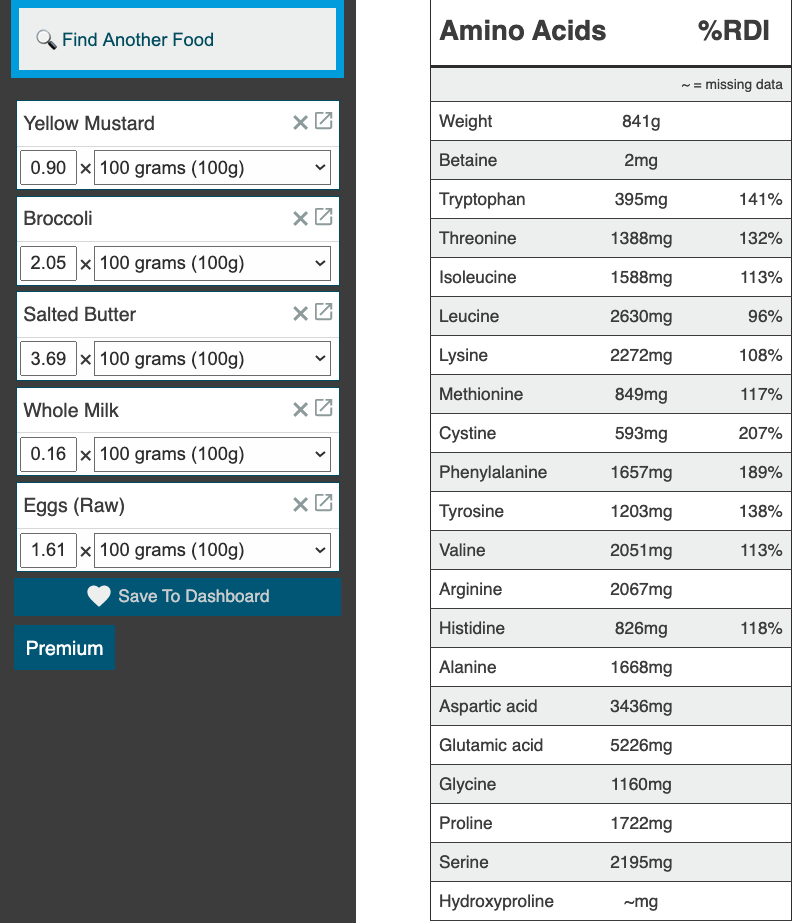
\includegraphics[width=.9\linewidth]{KBe20bio201retFoodDataProteinAminosDiet1.png}
\end{center}

\begin{enumerate}
\item \begin{quote}
Cross check the \url{https://www.myfooddata.com} (Links to an external
site.) essential amino acid values/food with the tables in the
slides (Links to an external site.). Do they seem consistent?
Provide evidence for you answer.
\end{quote}
\end{enumerate}

Well, we used the RDI from an external dataset. The my food data website
said that this was the data they used, but the RDI values were somewhat
different. However, the values the script comes up with are pretty
similar to the website, although our RDI seems to be higher than the
website.

\begin{enumerate}
\item \begin{quote}
Were there any essential amino acids, vitamins, or minerals needs
that were challenging to satisfy during your meal planning? What
are some foods particularly high in that vitamin or mineral?
\end{quote}
\end{enumerate}

Tryptophan and Methionine, which seems to be mostly taken care of by
milk and eggs.

\noindent\rule{\textwidth}{0.5pt}
\end{document}
